\documentclass{article}

\usepackage{fancyhdr}
\usepackage{extramarks}
\usepackage{amsmath}
\usepackage{amsthm}
\usepackage{amsfonts}
\usepackage{tikz}
\usepackage[plain]{algorithm}
\usepackage{algpseudocode}
\usepackage{enumerate}
\usepackage{amssymb}
\usepackage{mathtools}
\usepackage{float}
\usepackage{graphicx}
\usepackage{listings}

\graphicspath{ {./img} }

\usetikzlibrary{automata,positioning}

%
% Basic Document Settings
%

\topmargin=-0.45in
\evensidemargin=0in
\oddsidemargin=0in
\textwidth=6.5in
\textheight=9.0in
\headsep=0.25in

\linespread{1.1}

\pagestyle{fancy}
\lhead{\hmwkAuthorName}
\chead{\hmwkClass:\ \hmwkTitle}
\rhead{\firstxmark}
\lfoot{\lastxmark}
\cfoot{\thepage}

\renewcommand\headrulewidth{0.4pt}
\renewcommand\footrulewidth{0.4pt}

\setlength\parindent{0pt}
\setlength{\parskip}{5pt}

%
% Create Problem Sections
%

\newcommand{\enterProblemHeader}[1]{
    \nobreak\extramarks{}{Problem \arabic{#1} continued on next page\ldots}\nobreak{}
    \nobreak\extramarks{Problem \arabic{#1} (continued)}{Problem \arabic{#1} continued on next page\ldots}\nobreak{}
}

\newcommand{\exitProblemHeader}[1]{
    \nobreak\extramarks{Problem \arabic{#1} (continued)}{Problem \arabic{#1} continued on next page\ldots}\nobreak{}
    \stepcounter{#1}
    \nobreak\extramarks{Problem \arabic{#1}}{}\nobreak{}
}

\setcounter{secnumdepth}{0}
\newcounter{partCounter}
\newcounter{homeworkProblemCounter}
\setcounter{homeworkProblemCounter}{1}
\nobreak\extramarks{Problem \arabic{homeworkProblemCounter}}{}\nobreak{}

%
% Homework Problem Environment
%
% This environment takes an optional argument. When given, it will adjust the
% problem counter. This is useful for when the problems given for your
% assignment aren't sequential. See the last 3 problems of this template for an
% example.
%
\newenvironment{homeworkProblem}[1][-1]{
    \ifnum#1>0
        \setcounter{homeworkProblemCounter}{#1}
    \fi
    \section{Problem \arabic{homeworkProblemCounter}}
    \setcounter{partCounter}{1}
    \enterProblemHeader{homeworkProblemCounter}
}{
    \exitProblemHeader{homeworkProblemCounter}
}

%
% Homework Details
%   - Title
%   - Due date
%   - Class
%   - Section/Time
%   - Instructor
%   - Author
%

\newcommand{\hmwkTitle}{Homework\ \#2}
\newcommand{\hmwkDueDate}{Oct 22, 2024}
\newcommand{\hmwkClass}{MATH 173A}
\newcommand{\hmwkClassInstructor}{Professor Cloninger}
\newcommand{\hmwkAuthorName}{\textbf{Ray Tsai}}
\newcommand{\hmwkPID}{A16848188}

%
% Title Page
%

\title{
    \vspace{2in}
    \textmd{\textbf{\hmwkClass:\ \hmwkTitle}}\\
    \normalsize\vspace{0.1in}\small{Due\ on\ \hmwkDueDate\ at 23:59pm}\\
    \vspace{0.1in}\large{\textit{\hmwkClassInstructor}} \\
    \vspace{3in}
}

\author{
  \hmwkAuthorName \\
  \vspace{0.1in}\small\hmwkPID
}
\date{}

\renewcommand{\part}[1]{\textbf{\large Part \Alph{partCounter}}\stepcounter{partCounter}\\}

%
% Various Helper Commands
%

% Useful for algorithms
\newcommand{\alg}[1]{\textsc{\bfseries \footnotesize #1}}

% For derivatives
\newcommand{\deriv}[1]{\frac{\mathrm{d}}{\mathrm{d}x} (#1)}

% For partial derivatives
\newcommand{\pderiv}[2]{\frac{\partial}{\partial #1} (#2)}

% Integral dx
\newcommand{\dx}{\mathrm{d}x}

% Probability commands: Expectation, Variance, Covariance, Bias
\newcommand{\Var}{\mathrm{Var}}
\newcommand{\Cov}{\mathrm{Cov}}
\newcommand{\Bias}{\mathrm{Bias}}
\newcommand*{\Z}{\mathbb{Z}}
\newcommand*{\Q}{\mathbb{Q}}
\newcommand*{\R}{\mathbb{R}}
\newcommand*{\C}{\mathbb{C}}
\newcommand*{\N}{\mathbb{N}}
\newcommand*{\prob}{\mathds{P}}
\newcommand*{\E}{\mathds{E}}

\begin{document}

\maketitle

\pagebreak

\begin{homeworkProblem}
  Using the conditions of optimality, find the extreme points of the following functions and
  determine whether they are maxima or minima. You may use a computer to find the eigenvalues, but
  these questions should have easily accessible eigenvalues by hand.

  \begin{enumerate}[(a)]
    \item $f: \mathbb{R}^2 \to \mathbb{R}$ for $f(x_1, x_2) = x_1^4 + 2x_2^4 - 4x_1 x_2$
    
    \begin{proof}
      Note that
      \begin{gather*}
        \nabla f(x) = (4x_1^3 - 4x_2, 8x_2^3 - 4x_1) = 0 \\
        \nabla^2 f(x) = \begin{bmatrix}
          12x_1^2 & -4 \\
          -4 & 24x_2^2
        \end{bmatrix}.
      \end{gather*}
      Thus, the critical points are $x^* = (0, 0)$ or $(\pm 2^{-1/8}, \pm 2^{-3/8})$. We can then
      check
      \begin{gather*}
        \nabla^2 f(0, 0) = \begin{bmatrix}
          0 & -4 \\
          -4 & 0
        \end{bmatrix} \\
        \nabla^2 f(\pm 2^{-1/8}, \pm 2^{-3/8}) = \begin{bmatrix}
          12 \cdot 2^{-1/4} & -4 \\
          -4 & 24 \cdot 2^{-3/4}
        \end{bmatrix}.
      \end{gather*}
      Since the eigenvalues of $\nabla^2 f(0, 0)$ are $\pm 4$, $(0, 0)$ is a saddle point. Since
      $\det \nabla^2 f(\pm 2^{-1/8}, \pm 2^{-3/8}) = 128 > 0$ amd $\frac{\partial^2 f}{\partial
      x_1^2} > 0$, the critical points $(\pm 2^{-1/8}, \pm 2^{-3/8})$ are local minima.
    \end{proof}

    \item $f: \mathbb{R}^3 \to \mathbb{R}$ for $f(\vec{x}) = \vec{x}^T A \vec{x} + b^T \vec{x}$,
    where
    \[
    A = \begin{bmatrix}
    -1 & 0 & \frac{1}{2} \\
    0 & -1 & 0 \\
    \frac{1}{2} & 0 & -1
    \end{bmatrix}, \quad
    b = \begin{bmatrix}
    0 \\
    1 \\
    2
    \end{bmatrix}
    \]

    \begin{proof}
      \begin{gather*}
        \nabla f(\vec{x}) = 2A\vec{x} + b, \\
        \nabla^2 f(\vec{x}) = 2A.
      \end{gather*}
      Setting $\nabla f(\vec{x}) = 0$ yields
      \[
        \vec{x}^* = -\frac{1}{2} A^{-1} b = \begin{bmatrix}
          \frac{2}{3}\\
          \frac{1}{2} \\
          \frac{4}{3}
        \end{bmatrix}.
      \]
      Since the eigenvalues of $A$ are $-\frac{1}{2}, -1, -\frac{3}{2}$, we know $A \prec 0$ and the
      critical point is a local maximum.
    \end{proof}
  \end{enumerate}
\end{homeworkProblem}

\newpage

\begin{homeworkProblem}
  Consider the problem $f : \mathbb{R}^n \to \mathbb{R}$ for $f(x) = \|Ax - b\|_2^2$ for $A \in \mathbb{R}^{m \times n}$ and $b \in \mathbb{R}^m$. (Note: this was on the last homework). Write down the gradient descent algorithm to solve the optimization
  \[
  \min_{x \in \mathbb{R}^n} f(x).
  \]
  This doesn't have to be a computer program, just something of the form
  \begin{align*}
    x^{(0)} &= \dots \\
    x^{(t+1)} &= \dots (\text{where the right hand side is in terms of } x^{(t)}).
  \end{align*}

  

  \begin{proof}
    We already know $f$ is convex and the gradient of $f$ is
    \[
      \nabla f(x) = 2A^T(Ax - b).
    \]
    Thus, the gradient descent algorithm is
    \begin{align*}
      x^{(0)} &= \text{any vector from } \R^n \\
      x^{(t+1)} &= x^{(t)} - \mu^{(t)} \nabla f(x^{(t)}) = x^{(t)} - 2\mu^{(t)} A^T(Ax^{(t)} - b) \\
    \end{align*}
    where $\mu^{(t)} > 0$ and the terminating condition is of our choice.
  \end{proof}
\end{homeworkProblem}

\newpage

\begin{homeworkProblem}
  \textbf{Implementing Classification Model:} First some background for classification:
  \begin{itemize}
      \item You are given labeled data $\{(x_i, y_i)\}_{i=1}^N$ for $x_i \in \mathbb{R}^d$ and $y_i \in \{-1, 1\}$.
      \item Logistic regression involves choosing a label according to
      \[
      y = \text{sign}(\langle w, x \rangle).
      \]
      Note we ignore the $y$-intercept term here, so we only need the optimal $w \in \mathbb{R}^d$.
      \item It turns out the correct function to minimize to find the weights is
      \[
      F(w) = \frac{1}{N} \sum_{i=1}^N \log\left( 1 + e^{-\langle w, x_i \rangle y_i} \right).
      \]
  \end{itemize}
  \begin{enumerate}[(a)]
    \item Is $F(w)$ a convex function?
    \begin{proof}
      Note that
      \begin{gather*}
        \nabla F(w) = \frac{1}{N} \sum_{i=1}^N \frac{-y_i e^{-\langle w, x_i \rangle y_i}}{1 + e^{-\langle w, x_i \rangle y_i}} x_i  \\
        \nabla^2 F(w) = \frac{1}{N} \sum_{i=1}^N \frac{y_i^2 e^{-\langle w, x_i \rangle y_i}}{(1 + e^{-\langle w, x_i \rangle y_i})^2} x_ix_i^T.
      \end{gather*}
      Since the Hessian is positive semidefinite, $F(w)$ is convex.
    \end{proof}
    \item Find a gradient descent algorithm for minimizing $F$.
    \begin{proof}
      The gradient descent algorithm is
      \begin{align*}
        w^{(0)} &= \text{any vector from } \R^d \\
        w^{(t+1)} &= w^{(t)} - \mu^{(t)} \nabla F(w^{(t)}) = w^{(t)} - \frac{\mu^{(t)}}{N} \sum_{i=1}^N \frac{-x_i y_i e^{-\langle w^{(t)}, x_i \rangle y_i}}{1 + e^{-\langle w^{(t)}, x_i \rangle y_i}} \\
      \end{align*}
      where $\mu^{(t)}> 0$ and the terminating condition is of our choice.
    \end{proof}
  \end{enumerate}
\end{homeworkProblem}

\newpage

\begin{homeworkProblem}
  \textbf{Coding Question:} Recall that the equation for an ellipse in $\mathbb{R}^2$ is
  \[
    a_1x^2 + a_2y^2 = 1.
  \]
  Given data $\{(x_i, y_i)\}_{i=1}^N \subset \mathbb{R}^2$ that lie on (or near) the ellipse, you
  can find the best fit ellipse by solving
  \[
    \min_{\mathbf{a} \in \mathbb{R}^2} f(\mathbf{a})
  \]
  where
  \[
    f(\mathbf{a}) = \sum_{i=1}^{N} \left( a_1 x_i^2 + a_2 y_i^2 - 1 \right)^2.
  \]

  \begin{enumerate}[(a)]
    \item Find an $A \in \mathbb{R}^{N \times 2}$ and $b \in \mathbb{R}^N$ such that $f(\mathbf{a})
    = \|A \mathbf{a} - b\|_2^2$. What is $A$ in terms of $(x_i, y_i)$?

    \begin{proof}
      Put $A = \begin{bmatrix}
        x_1^2 & y_1^2 \\
        \vdots & \vdots \\
        x_N^2 & y_N^2
      \end{bmatrix}$ and $b = \begin{bmatrix}
        1 \\
        \vdots \\
        1
      \end{bmatrix}$ and we have
      \begin{align*}
        f(\mathbf{a}) &= \sum_{i=1}^{N} \left( a_1 x_i^2 + a_2 y_i^2 - 1 \right)^2 \\
        &= \sum_{i=1}^{N} \left( \begin{bmatrix}
          x_i^2 & y_i^2
        \end{bmatrix} \begin{bmatrix}
          a_1 \\
          a_2
        \end{bmatrix} - 1 \right)^2 \\
        &= \|A \mathbf{a} - b\|_2^2.
      \end{align*}
    \end{proof}

    \item Download the data provided on the HW page (called \texttt{HW2.ellipse.csv}), and create a
    scatter plot of the points (submit your code and the plot).

    \begin{center}
      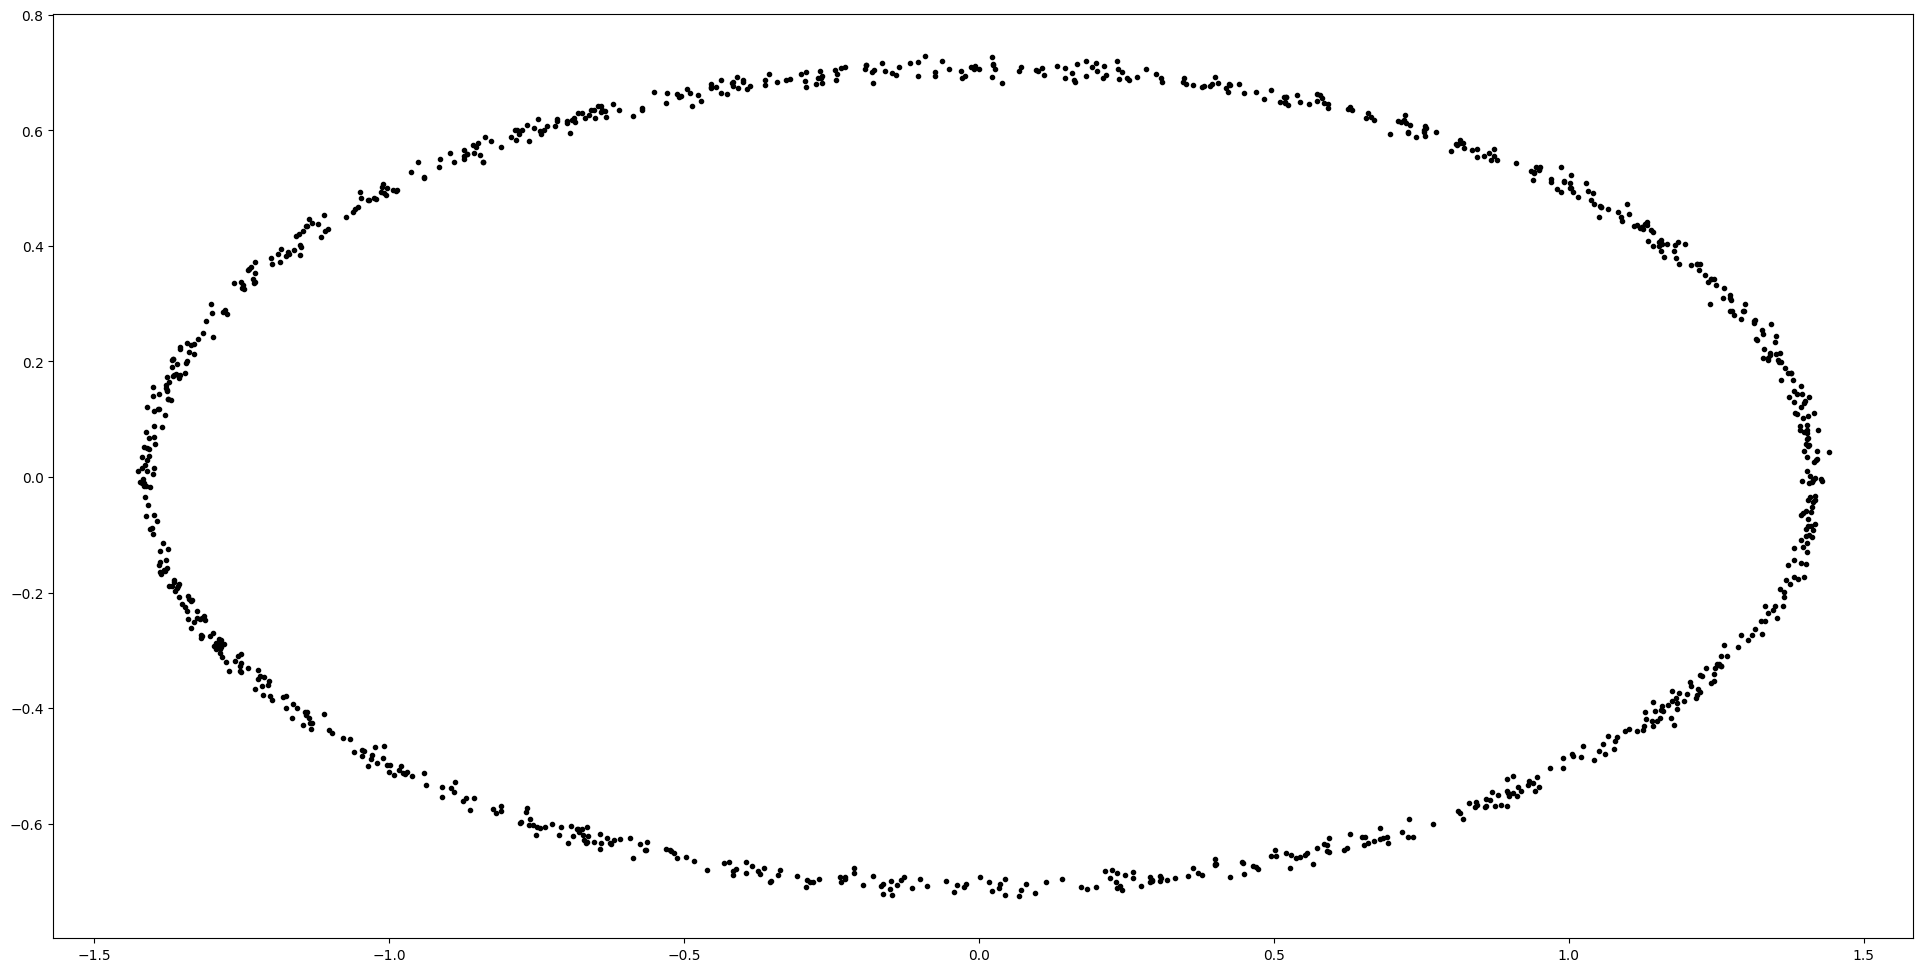
\includegraphics[width=.95\textwidth]{ellipse.png}
    \end{center}

    \textbf{Code:}

    \begin{lstlisting}[language=Python]
      ellipse = pd.read_csv('HW2_ellipse.csv', header=None)
      ellipse.columns = ['x', 'y']
      fig = plt.figure(figsize=(24, 12))
      ax = fig.add_subplot(1, 1, 1)  
      ax.plot(ellipse['x'], ellipse['y'], '.', color='black')
    \end{lstlisting}



    \item Using Problem 3, create computer code to compute the gradient descent algorithm on this
    $f(\mathbf{a})$. The code must include a stopping condition. Use a step-size of $\mu =
    \frac{1}{2 \|\mathbf{A}^T \mathbf{A}\|}$. Note, you cannot use a built-in gradient descent
    algorithm; it must be written with a while or for loop. Also note, the norm of a matrix
    $\|\mathbf{X}\| = \lambda_{\text{max}}(\mathbf{X})$ is the largest eigenvalue of $\mathbf{X}$,
    and can be computed using \texttt{norm(X,2)} in MATLAB or \texttt{np.linalg.norm(X,2)} in
    Python. (Submit the code)

    \textbf{Code:}

    \begin{lstlisting}[language=Python]
      A = ellipse.values * ellipse.values
      b = np.ones((A.shape[0], 1))
      mu = 1/(2 * np.linalg.norm(A.T @ A, 2))
      a = np.random.rand(2, 1)

      def df(x):
          return 2 * A.T @ (A @ x - b)

      for i in range(1000):
          a = a - mu * df(a)
    \end{lstlisting}


    \item Using the data provided and your gradient descent code, estimate the solution
    $\mathbf{a}$. Report $\mathbf{a}$ and $f(\mathbf{a})$. Given $f(\mathbf{a})$ and $N$, do you
    think you fit the data well or poorly? Given the convexity of $f$, do you think this is the
    optimal $\mathbf{a}$?

    \begin{proof}[Solution]
      The solution estimated by the code is $\mathbf{a} \approx \begin{bmatrix}
        0.5001 \\
        1.9946 \end{bmatrix}$, with $f(\mathbf{a}) \approx 0.4641$. Since we are given $N = 1000$
      points, on average each point is only off by $f(\mathbf{a})/N \approx 0.0004641$, which I
      think is borderline acceptable. Given that I believe $\mathbf{a}$ has reached a local minimum,
      $\mathbf{a}$ is a global minimum as $f$ is convex.
    \end{proof}
  \end{enumerate}

\end{homeworkProblem}
\end{document}